\chapter{Implementation}
\label{Implementation}
\textit{This chapter presents the implementation process of WebTaint. The chapter starts with a section describing \textit{\nameref{Policies}} enforced by the application. Thereafter a description of how  \textit{\nameref{souresSS}} were specified and lastly an explanation of the  \textit{\nameref{SoftwareArchitecture}} architecture.}



\section{Policies}
\label{Policies}
To be able to implement the functionality behind the taint tracker, security policies need to be defined. The security policies imply the principles and actions that the application strives to fulfill \parencite{BayukJenniferL2012Cspg}. The taint tracker developed in this thesis aims to fulfill two different kinds of policies. These are \textit{integrity} and \textit{confidentiality}.



\subsection{Integrity}
\label{Integrity}
The first policy is the integrity policy which is important as it defines that users may not modify data which they do not have permission to alter. The integrity policy aims to protect from, e.g., injections of malicious code that can lead to information disclosure or destruction of user data. To ensure this, we define the following policy:

\hfill
\begin{itemize}
    \item Users shall alter no data or execution without having the correct permission for the given data or execution.
\end{itemize}
\hfill

This entails that no information from untrusted sources shall pass through a trusted sink without first being sanitized.



\subsection{Confidentiality}
\label{Confidentiality}
The second policy is the confidentiality policy which defines that data given to the user should only be data that the user have the right to access. This goal concern the prevention of malicious usage where attackers wish to steal application data. To ensure this, we define the following policy:

\hfill
\begin{itemize}
    \item Users shall not gain access to data without having the correct permission for the given data.
\end{itemize}
\hfill

This policy entails that no information from confidential sources shall pass through a public sink unless it has the permission to do so.

\textit{While monitoring for confidentiality vulnerabilities are the sources, and sinks roles reversed compared to integrity flow analysis. The information wanted to protect is marked as sources and sinks are the systems public exit points.}



\subsection{WebTaint}
The two sections above state what both the integrity and the confidentiality policies of WebTaints aim to fulfill. The two policies can also be rewritten into policies for WebTaints internal logic. The internal policies are divided into the four tasks described in Table \ref{table:taintTracking} in Chapter \ref{Background}. These tasks are tainting, detainting, taint propagation, and assertion of non-tainted data.



\subsubsection{Tainting}
Table \ref{table:taintingpolicy} presents the tainting policies of WebTaint.

\begin{table}[H]
    \centering
    \caption{WebTaint's tainting policies.}
    \label{table:taintingpolicy}
    \begin{tabular}{rp{8.5cm}}
        \textbf{Integrity} & Data from untrusted sources shall always be marked tainted. \\
        \textbf{Confidentiality} & Data from private sources shall always be marked tainted. \\         
    \end{tabular}
\end{table}



\subsubsection{Detainting}
Table \ref{table:detaintingpolicy} presents the detainting policy of WebTaint.

\begin{table}[H]
    \centering
    \caption{WebTaint's detainting policy.}
    \label{table:detaintingpolicy}
    \begin{tabular}{rp{8.5cm}}
        \textbf{\begin{tabular}[c]{@{}r@{}}Integrity \&\\ Confidentiality\end{tabular}} & \begin{tabular}[c]{@{}l@{}}Data from sanitizers shall be marked as\\ detainted.\end{tabular} \\   
    \end{tabular}
\end{table}



\subsubsection{Taint Propagation}
Table \ref{table:propagationpolicy} presents the taint propagation policy of WebTaint.

\begin{table}[H]
    \centering
    \caption{WebTaint's taint propagation policy.}
    \label{table:propagationpolicy}
    \begin{tabular}{rp{8.5cm}}
        \textbf{\begin{tabular}[c]{@{}r@{}}Integrity \&\\ Confidentiality\end{tabular}} & \begin{tabular}[c]{@{}l@{}}Data resulting from tainted data shall be\\ marked tainted.\end{tabular} \\   
    \end{tabular}
\end{table}



\subsubsection{Assertion of Non-taint}
Table \ref{table:assertionpolicy} presents the assertion of non-tainted data policies of WebTaint.

\begin{table}[H]
    \centering
    \caption{WebTaint's assertion of non-taint policies.}
    \label{table:assertionpolicy}
    \begin{tabular}{rp{8.5cm}}
        \textbf{Integrity} & No untrusted data may pass through a trusted sink. \\
        \textbf{Confidentiality} & No private data may pass through a public sink. \\
    \end{tabular}
\end{table}



\section{Sources, Sinks \& Sanitizers}
\label{souresSS}
Defining the sources, sinks, and sanitizers is a large task in itself. There is no official documentation in Java specifying these for web applications. Depending on what application, framework, and library used the sources, sinks, and sanitizers will vary a lot. The sources, sinks, and sanitizers used in this thesis is, however, an aggregation from \textcite{sssCodeMaster} and \textcite{sssOWASP}. The web pages contain lists of sources, sinks, and sanitizers based on the author's experience in web application security. These lists are aggregated into one JSON file per each source, sink, and sanitizer containing classes and method names to instrument.



\section{WebTaint}
\label{SoftwareArchitecture}
The implementation of WebTaint was divided into three subprojects. The reasoning behind the separation was because of the need of transforming classes both before and during runtime as presented in Section \ref{Instrumentation}. These three projects are called Agent, Xboot, and Utils. The Agent handles the transformation in runtime and Xboot transforms the classes in the Base Java Runtime Environment. The logic of class transformation is the same in both projects and therefore centralized in the Utils subproject. A short description of the three subprojects is presented in Table \ref{table:subprojects}.

\begin{table}[H]
    \centering
    \caption{Description of the three subprojects in WebTaint.}
    \label{table:subprojects}
    \begin{tabular}{rp{10cm}}
        \textbf{Agent} & Running at runtime and triggering the transformation of sources, sinks, and sanitizers. \\
        \textbf{Xboot} & Running prior to runtime and transforming sources, sinks, sanitizers, String, StringBuilder, and StringBuffer in the Base Java Runtime Environment. \\
        \textbf{Utils} & Utilities to transform classes into sources, sinks, and sanitizers. \\
    \end{tabular}
\end{table}

Transformation of the String, StringBuilder, and StringBuffer classes is done in the Xboot project. This is done by transforming the classes to: 

\hfill
\begin{itemize}
    \item Contain a boolean to hold the taint flag.
    \item Propagate taint in each method and constructor (taint propagation policy \ref{table:propagationpolicy}).
\end{itemize}
\hfill

A high-level architecture of WebTaint instrumenting a web application is seen in Figure \ref{fig:WebTaint}. The Java Virtual Machine is un-instrumented, and so is WebTaint. The web application and all its depending libraries, however, are instrumented.

\begin{figure}[H]
    \centering
    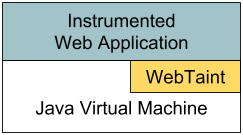
\includegraphics[width=0.4\textwidth]{images/WebTaintArchitecture.png}
    \caption{High-level architecture of WebTaint running on the JVM.}
    \label{fig:WebTaint}
\end{figure}

Out of the three subprojects, it is the Utils project that contains WebTaint's core logic. The Agent and Xboot act as a pipeline providing the Utils project with classes to analyze and possibly instrument. Therefore is only the logic behind the Utils project presented in the chapter below.

\subsection{The Utils Project}
The Utils project includes the core logic of marking methods as sources, sinks, and sanitizers. The significant part of the implementation is the same for the three different types, and the only difference is how they get instrumented. The logic behind finding the classes to instrument work by taking all classes and matching them with the three criteria in Table \ref{table:criterias}. This makes it possible to find if the class is a defined or builds upon a defined source, sink or sanitizer.

\begin{table}[H]
    \centering
    \caption{Description of the three criteria of finding sources, sinks and sanitizers to instrument.}
    \label{table:criterias}
    \begin{tabular}{rp{8cm}}
        \textbf{Is Class} & The class is listed as a source, sink or sanitizer. \\
        \textbf{Implements Interface} & The class implements interface of a listed source, sink or sanitizer. \\
        \textbf{Extends Class} & The class extends a class which [Is Class], [Implements Interface] or [Extends Class]. \\
    \end{tabular}
\end{table}

Classes found to be a source, sinks or sanitizer are instrumented by iterating through the class methods and comparing them with the methods defined in the JSON file corresponding to the matched source, sink or sanitizer. These matched methods will be instrumented depending on the type. What instrumentation is done per type is seen in Table \ref{table:instru}. 

\begin{table}[H]
    \centering
    \caption{Description of what logic is instrumented into the application depending on if the class method is a source, sink or sanitizer.}
    \label{table:instru}
    \begin{tabular}{rp{9.5cm}}
        \textbf{Source} & Tainting the current and return object (tainting policies \ref{table:taintingpolicy}). \\
        \textbf{Sink} & Asserting the current object and method arguments to be non-tainted (detainting policy \ref{table:assertionpolicy}) \\
        \textbf{Sanitizer} & Deainting the current and return object (detainting policy \ref{table:detaintingpolicy}). \\
    \end{tabular}
\end{table}

The instrumented logic of sinks is an assertion of the current object and arguments not to be tainted. If this assertion comes back incorrect is a remedial action needed. This action could be, a logging event, throwing a TaintException or modifying the tainted value into a safe predefined value. During the evaluations, the option of using a predefined value and logging the event is used.



\subsection{Limitations}
\label{NotableProblems}
One of the first problems that were introduced during the development of the application was that some classes could not be instrumented during runtime. More precisely, the classes that the Java Virtual Machine relies on can't be instrumented at runtime. However, the solution to this is to pre-instrument the Base Java Runtime Environment and create a new instrumented rt.jar file with statically modified versions of the classes. The created jar file loads through the option \textit{Xbootclasspath/p} \parencite{xboot} that appends the classes in the front of the bootstrap classpath. This triggers the Java Virtual Machine to utilize the instrumented rt.jar before the original version.

Another problem is that instrumentation of primitives and arrays is not possible. The implementation of WebTaint aims to support propagation of taint for Strings. However, the problem of not being able to instrument primitives and arrays creates the risk of possibly losing the taint when string operations are done with the help of byteArrays or charArrays. So, the solution to this is to create shadow variables as \textcite{BellJ.2014PIdd} did while developing Phosphor \parencite{phosphor}. However, another possible solution is to create a centralized memory bank just as \textcite{EnckWilliam2014Taif} did when implementing TaintDroid.

There is also the problem with primitive operations which are direct bytecode translations. Two examples of these are the usage of + (addition) and - (subtraction). Adding operations to these through Javassist's source level API is therefore not possible. Hence, solving these operations on bytecode level is therefore necessary. \parencite{Javassist}.